\documentclass[a4paper,man,natbib,floatsintext]{apa6}

\usepackage[english]{babel}
\usepackage[utf8x]{inputenc}
\usepackage{amsmath}
\usepackage{graphicx}
\usepackage[colorinlistoftodos]{todonotes}
\usepackage[font=small,labelfont=bf]{caption}
\newcommand{\rpm}{\raisebox{.2ex}{$\scriptstyle\pm$}}
\usepackage{amsmath}
\DeclareMathOperator*{\argmax}{arg\,max}

\title{Sherlock topic model paper}
% A common space for dynamic experiences and memories
% Geometric principles of episodic recall for naturalistic experiences
% The geometry of episodic recall for naturalistic experiences
% Recasting episodic memory as a weighted blend of prior experiences
% Capturing the moment-by-moment flow of information in naturalistic stimuli
% A continuous, content-general approach to characterizing memory for naturalistic events
% A common model for naturalistic stimuli, memories, and brains
% \title{A dynamic, content-general encoding signal to characterize memory for naturalistic stimuli}
% Topic models as a bridge between naturalistic stimuli, memories, and brains
% Automated analysis of memory for naturalistic stimuli using topic modeling
% Topic modeling as a link between videos and memories
% Topic models as a bridge between dynamic experiences and memories

\shorttitle{Your APA6-Style Manuscript}
\author{Andrew C. Heusser \& Jeremy R. Manning}
\affiliation{Dartmouth College}

\abstract{
}

\begin{document}
\maketitle

\section{Introduction}

\subsection{Results}

\begin{figure}[t!]
\centering
\includegraphics[width=1\textwidth]{figs/0_analysis_schematic.pdf}
\caption{\label{fig:schematic}Schematic of the analysis approach. For each moment of the video, text descriptions were manually generated. Three exemplary time points are displayed here.  Below the video descriptions are text samples from an example participant's verbal recall transcript.  We trained a topic model on the moment-by-moment video description text and transformed participant's recall transcripts using this same model. The bar charts display the resulting topic model weights for the video (in blue) and recall (in orange) for three example topic dimensions.}
\end{figure}

\subsubsection{A model to capture the moment-by-moment flow of information in naturalistic stimuli}
We fit a topic model to overlapping windows of manually annotated text descriptions of scenes from an episode of the BBC series, Sherlock. The text description contained details of the scene such as the characters, location, and a short summary of the scene (see \ref{fig:schematic} for example text, see \ref{sec:methods} for analysis details). We then transformed the text descriptions with the (same) topic model, resulting in a scene (1000) by topics (100) matrix where each row of the matrix represents a probabalistic mixture of topics discovered in that scene. We expanded this matrix from 1000 to 1976 timepoints by copying the vectors for scenes that spanned multiple TRs. As depicted in \ref{fig:model}a, the topics are sparse and change slowly over time. This gradual change was anticipated, since we used overlapping windows of text (50 sentences) as input to the model. The sparsity was also expected since the topic modeling approach we used (Latent Dirichlet Allocation) assumes a sparse Dirichlet prior. By eye, there are clear transitions from one topic `state' to the next, likely indexing scene transitions in the stimulus.  To get a better handle on this temporal structure, we computed the timepoint-by-timepoint correlation matrix of the video model (\ref{fig:model}b).  This correlation matrix reveals that the model has a strong, blocky structure along the diagonal.  Another interesting feature is that there is very little correlation between events (i.e. the off-diagonal values are small). This is an important feature of the model because the `event' representations are unique and highly discriminable.

\subsubsection{Projecting verbal recall into stimulus space}
After watching the episode, participants verbally recalled (in order) as much of the episode as they could.  We used the same topic model (fit with the text descriptions of the video) to transform participants' verbal recall transcripts (split by sentence in overlapping chunks of 10 sentences). The result was a sentences (range: X to X) by topics (100) matrix for each participant, where each row represented the estimated mixture of topics for a given window of sentences during recall. In order to average the recall models across participants, we resampled each model at the resolution of the video model (1976 timepoints). The individual models can be seen in Supp Fig X and the group average is plotted in \ref{fig:model}c. Note that the topics were derived solely from the text descriptions of the stimulus, and so the topic models estimated for recall are entirely dependent on the topics in the episode. In effect, this approach projects the recall transcripts into the video 'stimulus space', allowing us to quantify the dynamics of verbally reported memories as well as relate them to the experiences from which they were born.

Next, we investigated the temporal structure of the recall matrices. For each participant, we computed a timepoint-by-timepoint correlation matrix from the recall model. Like the video model, the recall correlation matrices exhibited blocky structure along the diagonal, albeit .

\begin{figure}[t!]
\centering
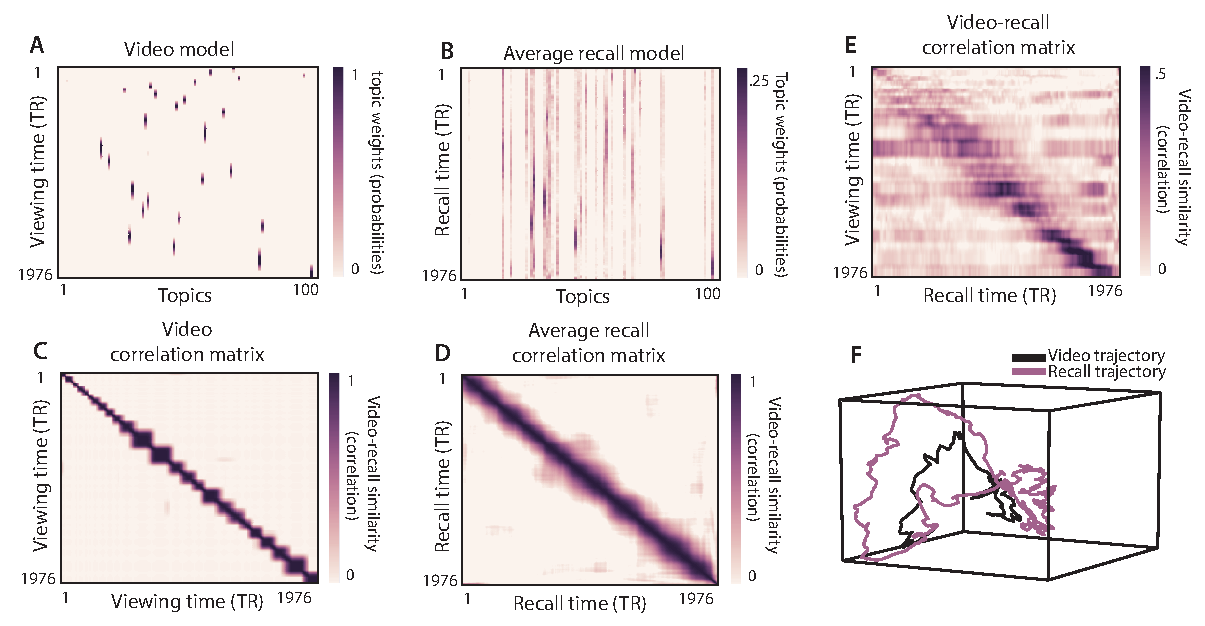
\includegraphics[width=1\textwidth]{figs/1_video_recall_models.pdf}
\caption{\label{fig:model}Topic models for the video and verbal recall. A. A timepoints (1976) by topics (100) matrix was created by fitting a topic model to overlapping segments of the moment-by-moment video text descriptions.  Each row represents the most likely mixture of topics for a given timepoint. Each columns represents a different topic. The darker the color, the higher the probability that the topic is contained in that timepoint. B. A timepoints (1976) by topics (100) matrix representing group average topic model of the recall transcripts.  All participant's recall transcripts were transformed using the topic model fit to the video descriptions and then resampled to the same length (1976). C. A viewing-time (1976) by recall-time (1976) correlation matrix representing the correlation of each moment of the video model with every moment of the average recall model. The darker the color, the higher the correlation between the video and recall models at a given timepoint. D. A 3D embedding of the video and recall topic models reduced using spectral embedding. }
\end{figure}

 However, the size/number of blocks varied across participants.  To quantify this structure, we estimated the number of recall `events' (k)  discovered in each participants' recall matrix (see Methods for details) using the event segmentation approach developed by Baldassano et al 2017.  Briefly, this algorithm implements a variant of a Hidden Markov Model to estimate a set of events (or states) given a multivariate time series and a k value (number of states). Figure X displays example correlation matrices for the participants with the lowest and highest k value.  We found that the estimated k value strongly correlated with the number of (hand-annotated) correctly remembered scenes across participants (Figure Xx, r=.67, p=.003). Thus, the blocky temporal structure of the recall matrices computed with our model is related to the variability in memory performance across participants.

Another interesting feature of the recall matrices is the off-diagonal structure, which represents the use of language that generalizes to more than one event. To characterize this aspect of the recall structure, we averaged the rows of the recall matrices according to the k events computed in the analysis described above.  This reduced the recall matrices from \# of sentences to k rows. Then, we computed k by k correlation matrices, representing the similarity of each event to each other event. To visualize these recall `networks', we embedded the k by topics matrices into a 2-dimensional space using Multidimensional Scaling (MDS), where each dot represents an event and the color of the dot represents the event index.  Then, we connected each event with a line where the color and line weight was proportional to the strength of the correlation between the events. These network plots can be seen in Fig X. To hypothesized that stronger correlations between recall events would

\subsubsection{Temporally aligning the stimulus and recall}
While most participants were able to recall most of the scenes in order, the rate of verbal description varied by participant and timepoint (Supp Fig X). Because of this participant-dependent non-linear relationship between stimulus and recall time, averaging the video-recall correlation plots across participants attenuates the robust within-participant effects. While further exploration of individual differences in recall rates is interesting, our primary goal here was to develop a model capable of accurately characterizing the content recovered during recall and explore how that varied across participants.  To that end, we leveraged dynamic time warping (DTW, REF) to temporally align the stimulus and recall matrices.  The algorithm returns a path of indices that bring the two timeseries into maximal temporal alignment (within constraints, see Methods for details).  For each participant, we computed the path and then warped the video model and recall model according to it. The length of the warp path varied by participant, and so the length (number of timepoints) of the warped video/recall matrices also varied by participant (range: X-X). To account for these differences, we resampled the timeseries back to the length of the stimulus (1976 time samples).

\begin{figure}[t!]
\centering
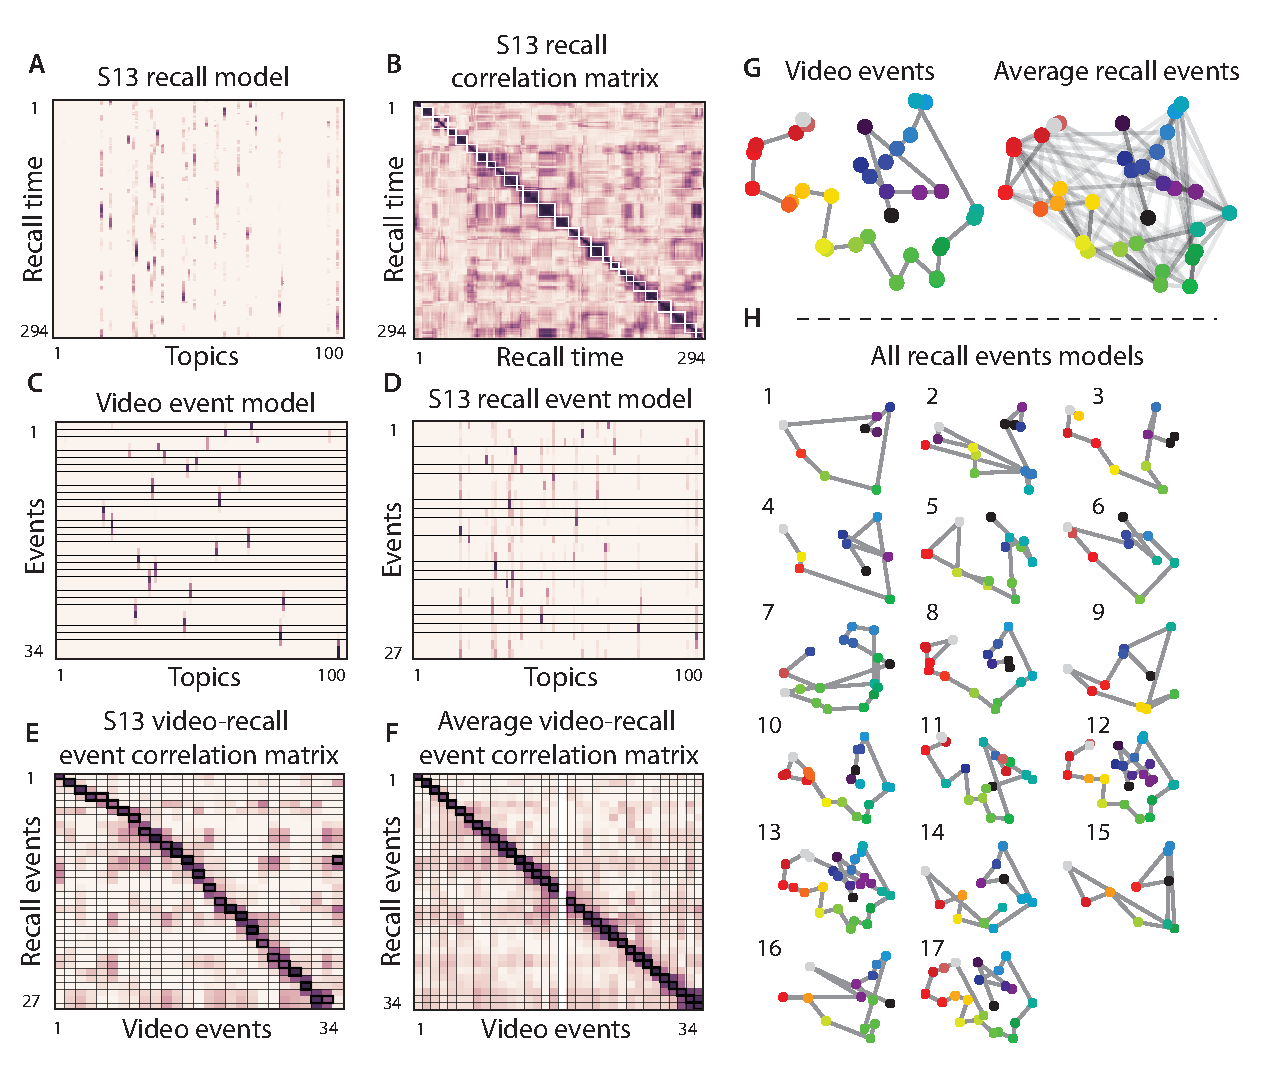
\includegraphics[width=.75\textwidth]{figs/2_eventseg.pdf}
\caption{\label{fig:eventseg} Event segmentation analysis of the video and recall models. A. A recall-time (294) by topics (100) matrix representing a recall model for a single participant (participant \#13).  B. A recall-time (294) by recall-time (294) correlation matrix for participant \#13. The white squares along the diagonal outline events, i.e. neighboring timepoints with a stable and similar topic vector. C. An events (34) by topics (100) matrix where each row represents the average topic vector for each event in the video model.  D. An events (27) by topics (100) matrix where each row represents the average topic vector for each event in the recall model. E. A recall events (27) by video events (34) correlation matrix representing the `match' between each video and recall event. The black squares identify the video event with the highest correlation to a given recall event. F. A group averaged recall events (34) by video events (34) correlation matrix.  The black squares identify the video event with the highest correlation to a given average recall event. G. 2D embeddings (reduced with UMAP algorithm) of each participants' recall event model (example shown in D). Each dot represents a recall event and the connecting lines indicate the order of recall. Colors indicate the most likely video event that the participant was describing as determined by the video-recall matching model.  H. 2D embedding of video and average recall event models.  }
\end{figure}


\subsubsection{Naturalistic extensions of classic memory analyses}

\begin{figure}[t!]
\centering
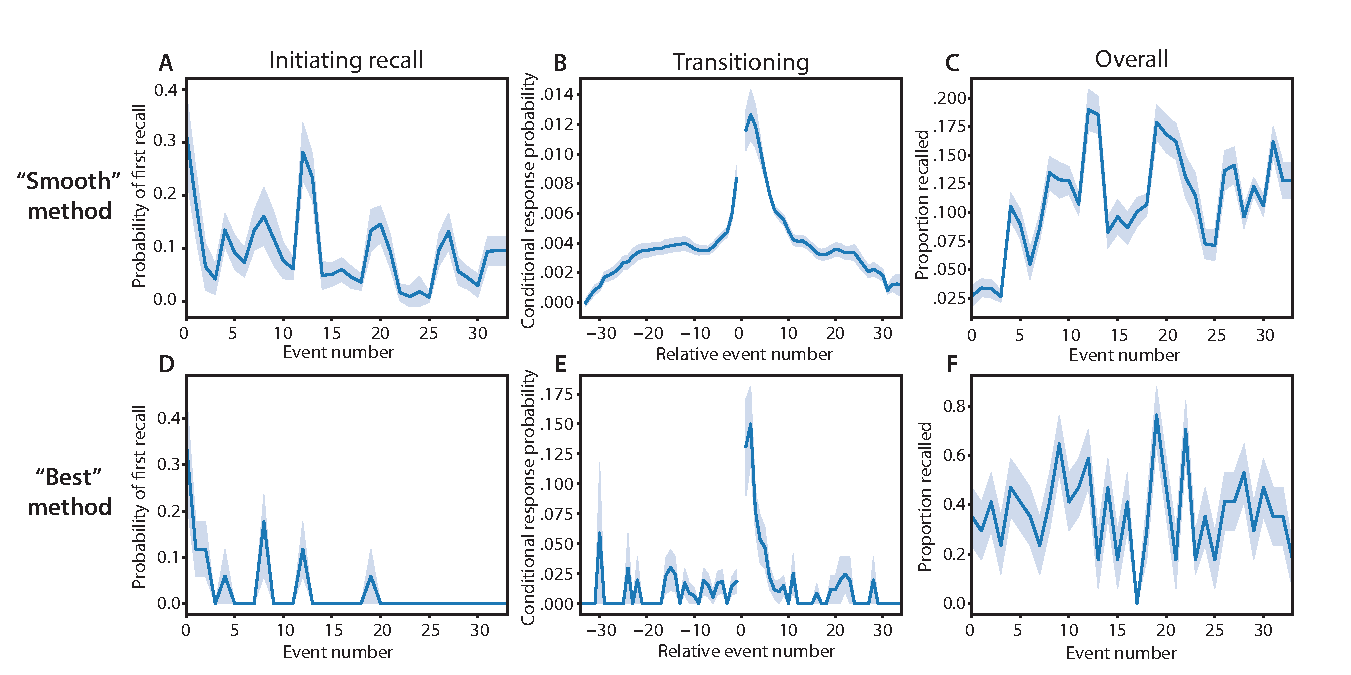
\includegraphics[width=1\textwidth]{figs/3_behav_eventseg.pdf}
\caption{\label{fig:behav}Naturalistic extensions of classic memory analyses. A-C use the `smooth' approach and D-F use the `best' approach (see Methods for details). A/D. The probability of first recall as a function of the serial position the the event during encoding. B/E. Given recall of event i, the probability that the next recalled item will be from serial position i \rpm~lag. C/F. Proportion recalled as a function of serial position. All error bars are the standard error of the mean derived from a bootstrap resampling procedure.
}
\end{figure}


\section{Methods}
\label{sec:methods}

\subsection{Participants and Experimental Design}
How much detail here? or just point to janice's paper?

\subsubsection{Fitting a topic model from text descriptions of Sherlock}
To quantify the flow of information from scene to scene, we used a topic model. A topic model estimates the most likely mixture of topics in a sample of text. First, the video was manually segmented into 1000 scenes, and a collection of descriptive features were manually transcribed.  For each scene, we considered the following features: scene details (i.e. a sentence or two describing what happened in that scene, space (indoor or outdoor), name of all the characters in the scene, name of the character in focus, name of the character speaking, location, camera angle, music presence, and words on the screen. We concatenated the text for all of these features within each segment, creating a 'bag of words' describing each scene. We then transformed the text descriptions into overlapping windows of 50 scene segments. For example, the first text sample comprised the text from the first 50 segments, the second comprised the text from n+1:n+51, and so on. We trained our model using these overlapping text samples using scikit-learn's `CountVectorizer' and `LatentDirichletAllocation' classes.  First, the text was transformed into a vector of word counts (default scikit-learn parameters). This gave a word count vector for each scene in the video.  Then, the word count vectors were used to fit a topic model (number of topics=100, method=batch).

\subsubsection{Projecting the video and verbal recall into a common space}
We used the model described above to transform the video text descriptions and verbal recall transcripts into a common space.  We created the video model by transforming exactly the same text (overlapping scene descriptions) with the topic model, resulting in a scene (1000) by topic (100) matrix that summarized the topics in each scene (Fig. \ref{fig:model}a). The scene descriptions often spanned multiple timepoints (i.e. TRs). To account for this, we expanded the video model by copying the rows of the model for as many timepoints that the scene description spanned. After this expansion, the shape of the model was the length of the duration of the video (1976 TRs).

To create the recall models, for each participant we tokenized the recall transcript into a list of sentences and then mapped the list to overlapping windows of 10 sentences.  We transformed the list of overlapping recall sentences using the model that was trained on the video text. The result of this was a matrix (\# of sentences by 100 topics) that represented the most likely mixture of topics for a given chunk of sentences. We resampled the recall model to be the same length as the video model (1976 samples). The result was 17 participant-specific recall models (1976 timepoints by 100 topics). Intuitively, if the recall transcript for a given participant correctly described each video scene in order, the video and recall models should match closely.  However, if the scenes were recalled out of order, omitted, or described using language that was very different from the video scene descriptions, the video and recall models would look very different. Figure \ref{fig:model}b shows the group average recall model. Qualitatively, the two matrices appear to be similar. Our next set of analyses sought to quantify this relationship.

To quantify the similarity between the movie and recall models, for each participant we correlated every moment of the video model with every moment of the recall models, resulting in a timepoints (1976) by timepoints (1976) correlation matrix for each participant.  The individual matrices for each participant can be seen in Supp Fig. X and the group average is displayed in \ref{fig:model}c.

\subsubsection{Estimating the number of recall events for each participant}
Our metric for choosing k was to select the value that maximized the ratio of the average `within-event' correlation (i.e. blocks of time the model identified as an event) and the average `across-event' correlation.

% \subsubsection{Accounting for nonlinearities between video and recall models}
% For many participants, the rate of recall changed over time (see Supp Fig X for an example). This becomes problematic if averaging the video/recall correlation matrices because the different recall rates distort the group average matrix. To correct for differences in recall rates across participants, we used dynamic time warping (DTW).  Briefly, DTW finds the path that maximizes the temporal alignment between two timeseries (REF). For each participant, we used DTW to temporally align the video model and the participant-specific recall model. Because the path is different for each participant, the length of the warped matrices varied across participants (range: X to X). To account for this, we resampled the matrices back to their original shape (1976 x 100).

\subsubsection{Characterizing memory performance}
We used a few different metrics to assess memory that were all designed to capture the relationship between the video and recall models.  First, to get a general sense for the match between the video and recall matrices, we vectorized the the matrices and correlated them.  This resulted in a single number representing how well a given participant recalled the video. To get a temporally dynamic measure of memory, for each participant we computed the pairwise correlation between matching video/recall timepoints.  This allowed us to assess memory for individual moments of the video. Finally to get a more nuanced representation of memory for the video, we computed a video/recall model correlation matrix for each participant. These timepoint (1976) by timepoint (1976) matrices represent the correlation between every moment of the video model and every moment of the recall model. To provide some intuition, if a participant recalled every scene at the same rate and in exactly the same order as the video, we would expect high correlation values along the diagonal of this matrix. However, if a participant recalls the scenes out of order, or at different rates for different scenes, this will result in high values off the diagonal.

% \subsection{fMRI analyses}
% Seventeen participants watched the first 50 minutes of Episode 1 of BBC's Sherlock. The video was split into two parts of approximately equal length (946 and 1030 TRs). All data were preprocessed and transformed to 3mm MNI space as described in the paper. Data were zscored across time at every voxel. 6mm smoothing was applied.
% Files are cropped so that all video-viewing data are aligned across participants, and all recall data are aligned to the scene timestamps below. The cropping includes a constant 3-TR (4.5 sec) shift to correct for hemodynamic lag.
%
% \subsubsection{Univariate subsequent memory analysis}
% To characterize brain regions involved in memory encoding, we conducted an analysis inspired by prior studies investigating the  `subsequent memory effect' (Paller and Wagner).  For each participant, we computed the correlation between topic vectors at each timepoint of the video model and recall model (they were temporally aligned with DTW and resampled to 1976 timesamples). The result was a 1 x 1976 vector of correlation values representing how similar each moment of the video model was to each moment of the recall model. Then, to compute the average correlation, we Fisher's z transformed the correlation vectors, averaged them together, and then inverse Fisher's z transformed them.  Finally, we mean centered the vector.  This 1 x 1976 vector represents memorable/unmemorable parts of the video, and be thought of as a `continuous' extension of a subsequent memory regressor.  We convolved the timeseries with a double gamma function (PARAMS) to account for the hemodynamic response, and used it as a model for each voxel's activity timeseries (using FSL software).  Finally, to aggregate across participants, we performed a mixed effects (ordinary least squares) analysis, thresholding at p<.001 and cluster correcting a p<.05.
%
% \subsubsection{Multivariate searchlight analyses}
% Our multivariate analyses were designed to capture brain regions whose timepoint-by-timepoint correlational structure mirrors the correlational structure of the video and recall topic models during video viewing. To that end, we conducted a searchlight analysis (5x5x5 voxel cube) where for each cube, we correlated the model timepoint-by-timepoint correlation matrix with the neural correlation matrix. To aggregate across participants, we computed Fisher's z transformed the correlations and then averaged.  To assess significance, we recomputed this group analysis 100 times, but randomly phase shifted the model (by \# of timepoints - 1) by the same amount for each participant but different amounts for each permutation to build a null distribution of correlation values. Finally, we thresholded the group averaged correlation maps where the `real' correlation value for a given voxel exceeded the 95th percentile of the null distribution.
%
% We first performed this analysis using the unwarped video model. Thus, the same model was applied to each participant and each searchlight cube. We then performed this analysis on the participant-wise recall models. To correct for non-linearities between the video model and recall models, for each participant we used DTW to temporally align the matrices. The algorithm recovers a path of coordinates that would bring the video and recall model in maximal temporal alignment. We used this path to warp the fMRI data and the recall model into alignment (separately for each participant). Then, we performed the exact same analysis as described above, using a searchlight to correlate the timepoint-by-timepoint recall and neural correlation matrices. The statistics for both analyses were computed as described above.

\subsection{References}

LaTeX automatically generates a bibliography in the APA style from your .bib file. The citep command generates a formatted citation in parentheses \citep{Lamport1986}. The cite command generates one without parentheses. LaTeX was first discovered by \cite{Lamport1986}.

% \subsection{Tables and Figures}

% Use the table and tabular commands for basic tables --- see Table~\ref{tab:widgets}, for example. You can upload a figure (JPEG, PNG or PDF) using the files menu. To include it in your document, use the includegraphics command as in the code for Figure~\ref{fig:frog} below.



\bibliography{memlab}

\end{document}

%
% Please see the package documentation for more information
% on the APA6 document class:
%
% http://www.ctan.org/pkg/apa6
%
